\section{Platform Parameter Design}
\label{sec:platform}

The microkernel slot size C, partition table size P and TDM table size in the control system design play a large role in task timing and scheduling. These parameters' units are shown in Table \ref{tab:design}. The mircokernel slot size will determine the the clock cycles (time) for which the microkernel needs to execute correctly, this was stated to be at least 40.96$\mu$s.

Thus the microkernel slot size could at best reach roughly 40 $\mu$s which would yield to about: $$ C_{min} = 100MHz \cdot 40.96 \mu s = 4096 \;\;Clock \; Cycles$$

This observation was small starting point of educated assumptions about which C and P to chose. Then it was decided rather than picking values for P and C separately to pick a fraction, relating those two. 

In Section \ref{sec:steps} the steps to the findings of sufficient values for P, C and TDM tabel size will be carried out. The goal is to meet the design constraints and at the same time have a good Quality of Control.

\subsection{Design and Workflow}
\label{sec:steps}
This subsection will discuss selection of P,C, Sensor to actuator delay and some choices considered for poles, TDM table size in order to meet the design constraints. To create an overview of how this was done, a timeline with the steps taken will be presented here.

\begin{figure}[h!]
	\begin{center}
		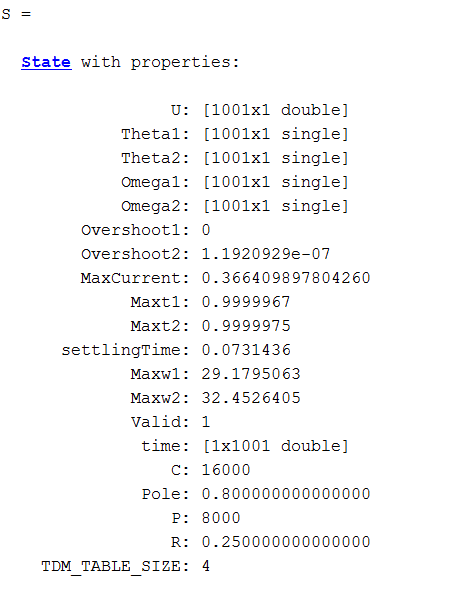
\includegraphics[width=0.5\linewidth]{img/S}
		\caption{State object of the system and its properties. This shows the values for the best solution found. The values will be explained throughout the report}
		\label{fig:S}
	\end{center}
\end{figure}

\begin{figure}[h!]
	\begin{center}
		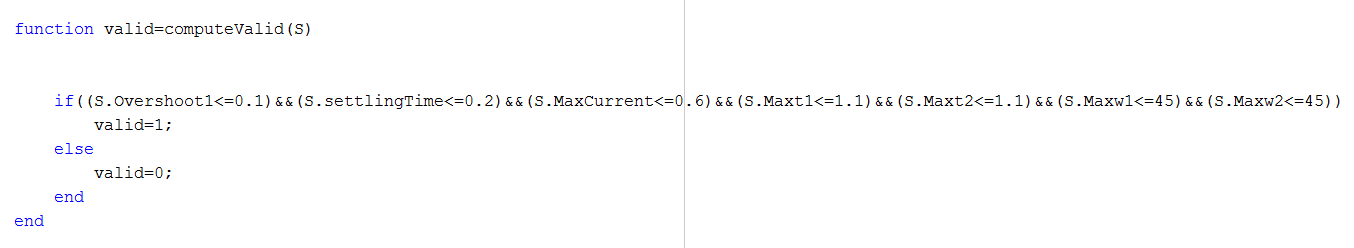
\includegraphics[width=1.1\linewidth]{img/valid}
		\caption{Performing design requirements condition on State Object.}
		\label{fig:valid}
	\end{center}
\end{figure}



\begin{enumerate}
	\item First tests made were rather basic and were used to determine the acuteness of poles on the system. A Matlab script was made to keep P=C,from 5000 up to 16000 clock cycles, and alternating the poles from 0.6 up to 0.9 with 0.1 as increment(keeping all poles at the same value). Along each test, settling time and validity of design constraints was included as output. Thus the valid parameter would render 0 or 1 depending on if all design constraints are met or not.
	
	To clarify all combinations of the following were tested, 40 in total:
	\begin{description}
		\item[P=C=] [5000:1000:16000]
		\item[Poles=] [0.6:0.1:0.9]$\cdot$[1 1 1 1 1]
		\item[TDM Table Size] = 4
	\end{description}
	When poles were at 0.6 and 0.7 there were very few valid options so these were excluded.
	
	\item Then ruling out poles at 0.6 and 0.7 and sticking to 0.8 and 0.8 where that gave more promising results. Then adding a fraction relation between C and P as shown here:
		\begin{description}
			\item[P=$\dfrac{C}{frac}$] where frac = [1:0.1:2]
			\item[Poles=] [0.8:0.1:0.9]$\cdot$[1 1 1 1 1]
			\item[TDM Table Size] = 4
		\end{description}
	This yielded around \textbf{200 options} both valid and invalid counted.
	\item Now filter out only valid results, which meet the design constraints set such as settling time and current limitations (and a few more). This is yielded to \textbf{102 valid options}.
	\item Next calculate the Quality of Control and R for each of the valid option which then allows for calculating a cost function(QoC/R) for each of the 102 options.
	\item Now all of the options chosen at this point are valid but the cost function will allow us to determine the most promising ones even though this done for a fixed TDM table size. Out of these 102, the top candidates were chosen and are investigated further, these are shown in Table \ref{tab:list}. The higher the ranking, the better the options is considered to be. Where options with pole at 0.8 are a bit more unstable when settling time is up, the best options representing poles at 0.9 was also chosen even though it considerable worse ranking it proofs to be more stable.
	
	\begin{table}[htbp]
		\centering
		\caption{Options for platform parameters derived from numerous investigations and scripts. Higher ranking indicates overall better performance. Poles are chosen identical for all five of them. TDM table size it constant at 4.}
		\begin{tabular}{lllccccc}
			\toprule
			Rank & C& P & Poles &Valid &OoC & R & $\dfrac{QoC}{R}$ [Cost Function] \\ 
		\midrule
		\textbf{102} & \textbf{16000} & \textbf{8000} & \textbf{0.8} & \textbf{{1}} & \textbf{\textcolor{blue}{18.34}} & \textbf{0.2500} &\textbf{ 73.34} \\ 
		101 & 15000 & 7895 & 0.8 & 1 & 18.39 & 0.2586 & 71.11 \\ 
		100 & 16000 & 8421 & 0.8 & 1 & 18.34 & 0.2586 & 70.90 \\ 
		99 & 8000 & 4000 & 0.9 & 1 & 17.51 & 0.2500 & 70.05 \\ 
		\textbf{{98}} & \textbf{{}} & \textbf{{3500}} & \textbf{{0.9}} & \textbf{ {1}} &\textbf{ \textcolor{blue}{17.51}} & \textbf{{0.2500}} & \textbf{{70.05}} \\ 
		97 & 15000 & 8333 & 0.8 & 1 & 18.39 & 0.2679 & 68.65 \\ 
		96 & 10000 & 5000 & 0.9 & 1 & 17.12 & 0.2500 & 68.49 \\
		\midrule 
		\textbf{21} & \textbf{16000}& \textbf{8000}& \textbf{0.9}&\textbf{{1}}&\textbf{\textcolor{blue}{8.10}}&\textbf{{0.2500}}&\textbf{{32.38}}\\
		
	\midrule
	\end{tabular}
	\label{tab:list}
\end{table}



	\item Now when some good values for P, C and the poles had been chosen it is a good time to look at the TDM table sizes. This is also covered in more detail in Section \ref{sec:codesign}.


\end{enumerate}

\subsubsection{Sensor to actuator delay}
\label{sec:stad}

The sensor to actuator delay is the time in the control system it takes from sensor input until computed and actuator actuates. This time is then highly related to P, C, TDM table size, Global clock frequency and sampling period. The exact delay can be precisely calculated per Equation \ref{eq:delay}. And number are put in according to one of the options determined for the controls system from Table \ref{tab:list}.

\begin{equation}
	\text{Exact Delay}=(C+P)\cdot NUMTASKS  = (16000+8000)\cdot 3  = 72000 \text{ clock cycles}
	\label{eq:delay}
\end{equation}
\begin{equation}
	\text{Rounded Delay}= \text{ceil}\left(\dfrac{\text{Exact Delay}}{\text{Plant Sampling Period}}\right) \cdot \text{Plant Sampling Period} = 80000 \text{ clock cycles}
\label{eq:rounddelay}
\end{equation}

\begin{equation}
\text{Delay}=\text{Rounded Delay} - \text{Exact Delay}= 8000 \text{ clock cycles}
\label{eq:delayall}
\end{equation}

Then when substituting 8000 for the delay in sconfig.c the output file gave error regarding timing that the delay might be to long. The reason might be because the delay landed just on the other side of the next task so reducing the delay to 7000 clock cycles did the trick and the results matched the Simulink results.

%\subsection{Implementation of Design steps in Matlab}
%\color{red}
%Show Matlab code for designing and explain matlab approach. Would be great if you, Sai, could just put some code snippets from matlab. Like some part of the looptrhough code where the valid parameters is gotten for example or your cool objects ;).
%\color{black}

%\begin{lstlisting}[language=matlab,caption={Matlab code showing the loopthrough function }]
%Matlab code
%\end{lstlisting}


